% platex report && dvipdfmx report.dvi && open report.pdf
\documentclass{jsarticle}
\usepackage{listings,jlisting}
\usepackage[dvipdfmx]{graphicx}
\usepackage[hang,small,bf]{caption}
\usepackage[subrefformat=parens]{subcaption}
\captionsetup{compatibility=false}
\lstset{
  basicstyle={\ttfamily},
  identifierstyle={\small},
  commentstyle={\smallitshape},
  keywordstyle={\small\bfseries},
  ndkeywordstyle={\small},
  stringstyle={\small\ttfamily},
  frame={tb},
  breaklines=true,
  columns=[l]{fullflexible},
  numbers=left,
  xrightmargin=0zw,
  xleftmargin=3zw,
  numberstyle={\scriptsize},
  stepnumber=1,
  numbersep=1zw,
  lineskip=-0.5ex
}

\begin{document}

\title{情報システム論実習 演習課題 5月19日分}
\author{6930318812 沖野 雄哉}
\maketitle

\begin{figure}[h]
 \begin{minipage}[b]{0.50\linewidth}
  \centering
  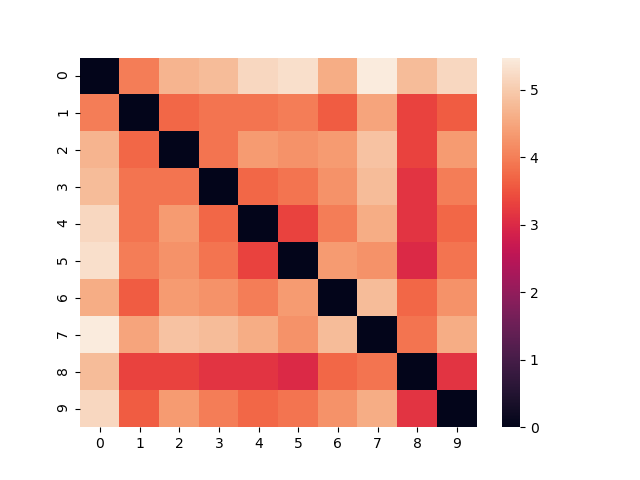
\includegraphics[keepaspectratio, scale=0.42]
  {./euclidean_distance_bows.png}
  \subcaption{ユークリッド距離, BoW}\label{euclidean_bow}
 \end{minipage}
 \begin{minipage}[b]{0.50\linewidth}
  \centering
  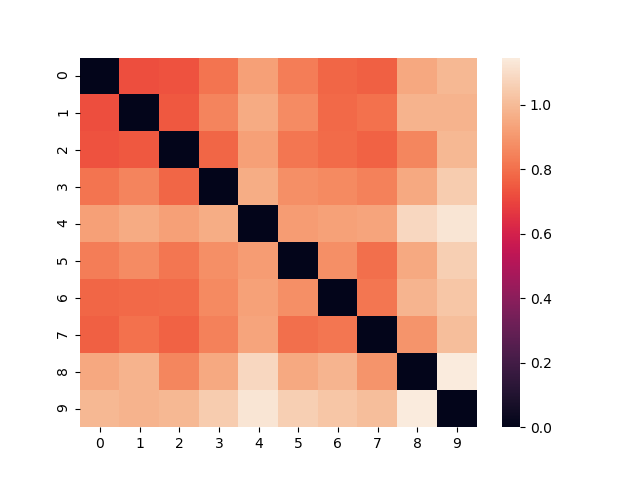
\includegraphics[keepaspectratio, scale=0.42]
  {./euclidean_distance_tfidfs.png}
  \subcaption{ユークリッド距離, tf-idf}\label{euclidean_tfidf}
 \end{minipage}
 \begin{minipage}[b]{0.50\linewidth}
  \centering
  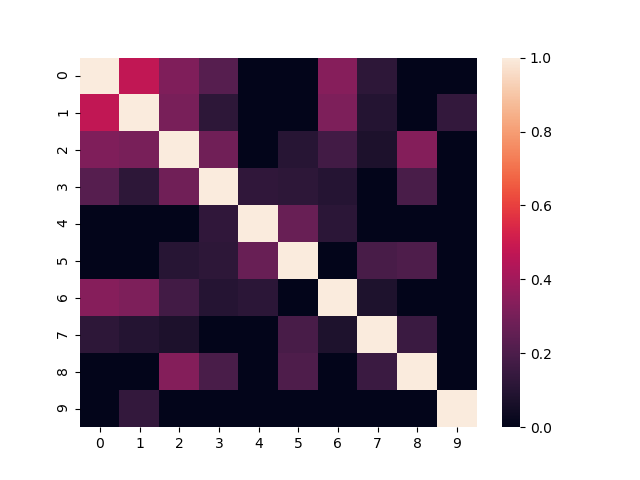
\includegraphics[keepaspectratio, scale=0.42]
  {./cosine_similarity_bows.png}
  \subcaption{コサイン類似度, BoW}\label{cosine_bow}
 \end{minipage}
 \begin{minipage}[b]{0.50\linewidth}
  \centering
  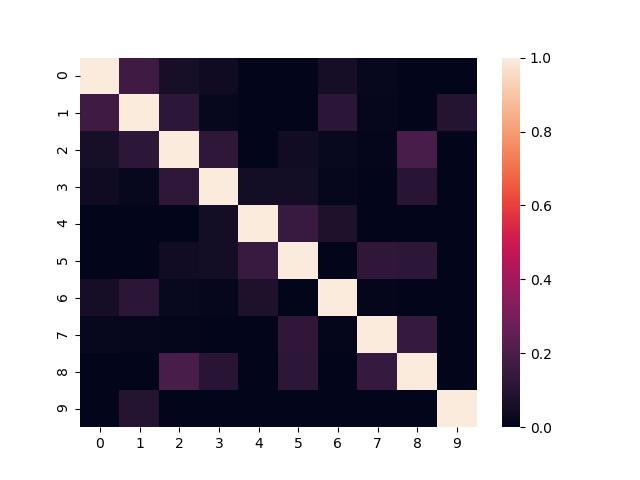
\includegraphics[keepaspectratio, scale=0.42]
  {./cosine_similarity_tfidfs.png}
  \subcaption{コサイン類似度, tf-idf}\label{cosine_tfidf}
 \end{minipage}
\end{figure}

\end{document}
